\section{Libraries}

\texttt{Dash}, the library I used for the graphic interface, works with \texttt{Plotly} for the graphs, which in turn is easy to use together with \texttt{Pandas} for 
data handling.

\begin{figure}[!ht]
    \centering
    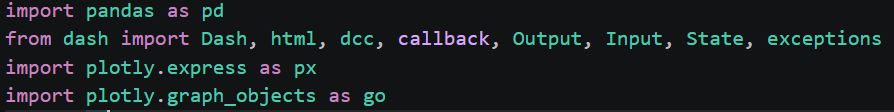
\includegraphics[width = 0.85\textwidth]{Img/import.png}
    \caption{Libraries: Dash, Plotly, Pandas}
    \label{import}
\end{figure}

\subsection{Brief overview of Dash}
\texttt{Dash} allows to create a web app (run from the browser). Its structure is encoded in the "layout" function, and is made of several "components", which can 
either be \texttt{html} components or \texttt{Dash} core components (\texttt{dcc}). The layout syntax is

\begin{lstlisting}[language = Python]
    def serve_layout():
        return html.Div([
        ...
        ])
\end{lstlisting}

and all the layout components go inside the \texttt{html.Div} (the \texttt{html.Div} structure is a "box" that can be nested arbitrarily). Every component has associated 
properties, which for example can be a \texttt{value} (i.e. a normal python variable) or a \texttt{children} (a subcomponent). The component properties can be accessed via 
the component \texttt{id}, which is a string that identifies it.  Among the \texttt{ash} core components are structure for input/output such as \texttt{dcc.Dropdown}, \texttt{dcc.RadioItems} etc., 
and also the \texttt{dcc.Graph} component, whose property is of type \texttt{figure}, which is to say a \texttt{Potly.graph{\textunderscore}objects.Figure} variable. \\

The user interaction happens through the \texttt{callback} functions. \texttt{callback} is a function decorator, which means it's a function that takes other functions as input 
and calls them inside their definition, while also performing other actions; \texttt{Dash} callbacks are applied to their argument functions with the following syntax,

\begin{center}
    \begin{lstlisting}[language = Python]
    @callback(
        # Input and output
        ...
    )
    def function(...): # argument function
        ... 
    \end{lstlisting}
\end{center}


or, in the case of long callbacks (needed when the running time of the argument function is longer than $30 \, \mathrm s$),

\begin{center}
    \begin{lstlisting}[language = Python]
    @app.long_callback(
        output = [
            ...
        ]
        inputs = [
            ...
        ]
        ...
        manager = ... 
    )
    def function(...):
        ...
    \end{lstlisting}
\end{center}


The inputs and outputs of the callbacks are specified by the \texttt{id} of layout components: when the properties are changed by user input or any other way, the 
callback is called, and it passes the component properties to its argument function.

\subsection{Notable comments on the implementation}

\begin{itemize}
    \item At the definition of a callback, its inputs, outputs and states are specified. Inputs are \texttt{Dash} components that trigger the callback upon their modification; 
    outputs are \texttt{Dash} components that are returned to the layout at the end of the callback; states are \texttt{Dash} components which the callback can access (and 
    on which it depends), but that don't trigger the callback. Since many callbacks require multiple inputs (e.g. the callback for creating the interference patterns 
    needs the range of the filtering width, the range of the slits separation and the type of filtering, as shown in fig. \ref{patpar}), in order to avoid triggering the 
    callback at each modification, most parameters are passed as states, and a single confirmation button is the actual input. The property of "button" components is of 
    type \texttt{n{\textunderscore}clicks}. 
    \item Some of the callbacks (generation of speckle field, interference, automatic analysis) require more than $30 \, \mathrm s$, therefore it was necessary to use 
    \texttt{long{\textunderscore}callback}.
    \item By default, every callback is triggered at the opening of the app; the standard way to avoid that (since for example it's possible that the function needs to read data 
    stored in external files that may not have been generated yet) is to raise a \texttt{PreventUpdate} exception if \texttt{n{\textunderscore}clicks = 0}.
    \begin{figure}[!ht]
        \centering
        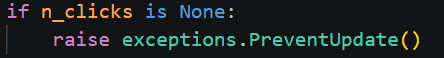
\includegraphics[width = 0.55\textwidth]{Img/prevent.png}
        \caption{Raising \texttt{PreventUpdate} exception}
        \label{prevent}
    \end{figure}
    \item In order to increase the modularity and ease of use of the app, all the data (simulated speckles fields and inteference patterns) are stored in \texttt{.csv} files 
    and accessed later (the speckles fields are accessed by the function for creating interference patterns, the patterns are accessed by the functions for data analysis): this 
    way the different steps can be executed independently. The same principle is applied to other parameters (setup parameters, average intensity of the fields, numerical 
    size of the statistical ensemble) that are stored in a \texttt{.json} file. 
    \item The \texttt{html.Div} component has a \texttt{ClassName} argument, that if defined can be used in a \texttt{.css} file to define its appearance 
    (size, color, margin\dots).
\end{itemize} 


% long callbacks?
% store data in external file because dash
% states
% prevent update
% css
% tabs?